\documentclass{pre-tfg}

\usepackage{listings}
\usepackage{longtable}
\usepackage{formular}
\usepackage{mathtools}
\usepackage[pdftex]{graphicx}
\usepackage{rotating}
\usepackage[utf8]{inputenx}
\usepackage[T1]{fontenc} % Codificación de salida 
\usepackage{marvosym}
\showhelp  % comenta o borra para eliminar ayudas

\title{Mooma, un procesador de máquinas de Moore}
\author{Javier Córdoba Romero, Juan José Corroto Martin y Fernando Vallejo Banegas}
%\advisorFirst{(nombre y apellidos)}
\advisorDepartment{Procesadores de Lenguajes}
%\advisorSecond{}
%\intensification{(INTENSIFICACIÓN)}
\docdate{2019}{Enero}


\DeclareGraphicsExtensions{.pdf,.png,.jpg}

\usepackage{color}
\definecolor{gray97}{gray}{.97}
\definecolor{gray75}{gray}{.75}
\definecolor{gray45}{gray}{.45}

\lstset{ frame=Ltb,
     framerule=0pt,
     aboveskip=0.5cm,
     framextopmargin=3pt,
     framexbottommargin=3pt,
     framexleftmargin=0.4cm,
     framesep=0pt,
     rulesep=.4pt,
     backgroundcolor=\color{gray97},
     rulesepcolor=\color{black},
     %
     stringstyle=\ttfamily,
     showstringspaces = false,
     basicstyle=\small\ttfamily,
     commentstyle=\color{gray45},
     keywordstyle=\bfseries,
     %
     numbers=left,
     numbersep=15pt,
     numberstyle=\tiny,
     numberfirstline = false,
     breaklines=true,
     keepspaces=true,
   }

% minimizar fragmentado de listados
\lstnewenvironment{listing}[1][]
   {\lstset{#1}\pagebreak[0]}{\pagebreak[0]}

\lstdefinestyle{consola}
   {basicstyle=\scriptsize\bf\ttfamily,
    backgroundcolor=\color{gray75},
   }

\lstdefinestyle{C}
   {language=C,
   }


\renewcommand*\lstlistingname{Listado}

\begin{document}

\maketitle
\tableofcontents

\newpage
\section{Descripción del Problema}
En este proyecto nos enfrentamos a un problema en el cual se nos pide crear un procesador de lenguaje para cierto Lenguaje de definición de máquinas Moore. Para ello vamos a necesitar la implementación de tres analizadores: léxico, sintáctico y semántico
,es decir, para este proyecto primero necesitamos crear un lenguaje para la definición de máquinas de Moore, y respecto a ese lenguaje va a trabajar nuestro “traductor”, el cual será capaz de originar la misma máquina de Moore pero en un lenguaje distinto, lenguaje objeto (JAVA).
Debido a que este proyecto abarca todo el proceso de la creación de un procesador de lenguaje podemos centrarnos en aprender, de forma práctica, el uso de los procesadores de lenguaje, ya que el dominio del problema (Máquinas de Moore) nos es conocido a todos. 

Una máquina de Moore es un tipo de máquina secuencial en la que la respuesta solo depende del estado actual de la máquina y es independiente de la entrada.
Una máquina de Moore es una estructura de la forma:
$Mo = (Q, Ent, Sal, tran, res, q_0)$
Siendo:
\begin{itemize}
    \item $Q$: conjunto de estados
    \item $Ent$: alfabeto de entrada
    \item $Sal$: alfabeto de salida
    \item $tran$: $ Q x Ent \rightarrow Q$, funcion de transicion
    \item $res$: $Q \rightarrow Sal$, funcion de respuesta
    \item $q_0$: estado inicial
\end{itemize}
\bigskip
Como podemos ver en el ejemplo [\ref{fig:MooreMachineExample}] una Máquina de Moore es un autómata compuesto de estados (representados por letras mayúsculas) asociados a una salida (en este caso un número que se encuentra separado del nombre del estado por una barra ``\slash'') y transiciones típicas entre estados.
\begin{figure}[htb]
	\centering
	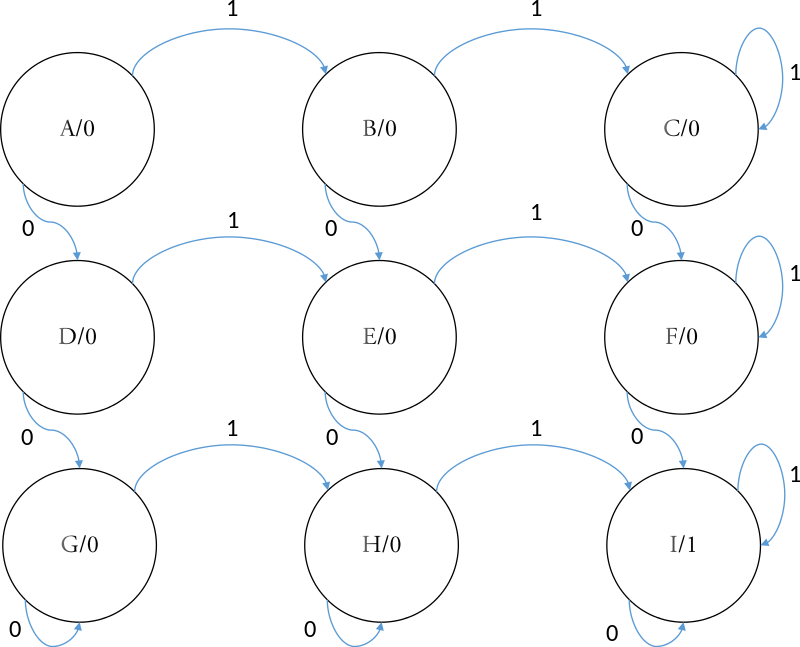
\includegraphics[width=10cm]{Moore_Machine.png}
	\caption{Ejemplo de Máquina de Moore.}
	\label{fig:MooreMachineExample}
\end{figure}
En este ejemplo la salida cambia a 1 y permanece así cuando al menos la cadena: ``0011'' aparece en la entrada (estado I). En el resto de estados la salida es 0.

\section{Lenguaje Mooma}
Para crear estas Máquinas de Moore hemos hecho un lenguaje específico de Dominio al que hemos llamado ``Mooma'' [\ref{fig:EBNF}].

\begin{lstlisting}[caption=EBNF de nuestro lenguaje de definición de Máquinas de Moore (Mooma)., label=fig:EBNF]
PROGRAM ::= [ENVIRONMENT] {OUTPUT} {DEFINE} {AUTOMATON};
ENVIRONMENT ::= "environment" ":=" {LETRA} ";";
DEFINE ::= "define" IDENT "{" ENTRADA ";" SALIDA ";" "}";
AUTOMATON ::= "automaton" IDENT "(" IDENT ")" "{" STATES ";" INITIAL ";" TRANSITIONS "}";
ENTRADA ::= "in" ":=" {EVENTO","}[EVENTO];
SALIDA ::= "out" ":=" {IDENT","}[IDENT];
STATES ::= "states" ":=" [{IDENT "|" EVENTO,}] IDENT "|" EVENTO;
INITIAL ::= "initial" ":=" IDENT;
TRANSITIONS ::= "transitions" "{" {IDENT "|" {EVENTO,}EVENTO "->" IDENT ";"} "}";
IDENT ::= LETRA {LETRA|DIGITO};
LETRA ::= "A" | "B" | "C" | "D" | "E" | "F" | "G"
       | "H" | "I" | "J" | "K" | "L" | "M" | "N"
       | "O" | "P" | "Q" | "R" | "S" | "T" | "U"
       | "V" | "W" | "X" | "Y" | "Z" | "a" | "b"
       | "c" | "d" | "e" | "f" | "g" | "h" | "i"
       | "j" | "k" | "l" | "m" | "n" | "o" | "p"
       | "q" | "r" | "s" | "t" | "u" | "v" | "w"
       | "x" | "y" | "z" ;
DIGITO ::= "0" | "1" | "2" | "3" | "4" | "5" | "6" | "7" | "8" | "9" ;
EVENTO ::= (1|2|3|4|5|6|7|8|9){DIGITO};
OUTPUT ::= IDENT ":=" CODIGO ";";
CODIGO ::= "{:" {ASCII} ":}";
COMMENT ::= "/*" {ASCII} "*/";

\end{lstlisting}
Un dato importante para tener en cuenta es que nuestro lenguaje trabaja con eventos, es decir la creación del diccionario de correspondencia entre eventos y las entradas del problema ha de ser diseñado por el usuario para la comprensión del resultado.

Los programas Mooma se encuentran divididos en cuatro partes: 
\begin{enumerate}
    \item Declaración del entorno, aquí se incluirá una construcción que comenzará por ''environment'' seguido del nombre o ruta del archivo que contiene el entorno (una clase Java que implementa una interfaz creada por nosotros, y que el usuario debe crear).
    \item  Código asociado a las salidas de los estados, que necesitará un identificador para poder ser usado posteriormente en la parte de declaración de entradas y salidas (marcado con \emph{define}) y la declaración del autómata (marcado con \emph{automaton}).
    \item Declaración de entradas y salidas (eventos y código). Aquí se incluirá una construcción que empieza con la palabra ``define'', seguido de un identificador, y se definirán un alfabeto de entrada (Recordamos que este alfabeto siempre consistirá en números que denotan eventos), y un alfabeto de salida. Este alfabeto de salida será una serie de identificadores definidos anteriormente, y denotan fragmentos de código en java que serán ejecutados como salida de un estado.
    \item Declaración de un autómata concreto. Ésta será otra construcción que empezará con la palabra ``automaton'' y, entre paréntesis, el identificador de una construcción “define” (Lo cual denotará los alfabetos de entrada y salida del autómata). Dentro de la construcción se incluirán el conjunto de estados del autómata junto con el identificador de su salida asociada, el estado inicial y una lista con las transiciones entre estados del autómata.
\end{enumerate}

Además, nuestro lenguaje tiene la opción de añadir comentarios empezando por ``\slash*'' y terminando por ``*\slash'', pudiendo poner cualquier cosa entre esas dos cadenas.

El \textit{Environment} no es obligatorio. En el \textit{Environment} se puede implementar la función translate, encargada de traducir la entrada que el usuario quiere que tenga la máquina de Moore en eventos, que es lo que la máquina tendrá como lenguaje de entrada. En el apartado de ejemplos se podrá ver mejor el uso del \textit{Environment}.

\subsection{Tabla de Tokens}

La tabla de tokens del lenguaje Mooma [\ref{tab:Tokens}] contiene todos los tokens del lenguaje junto con un patrón que lo define y un lexema de ejemplo. En azul se pueden observar las palabras reservadas del lenguaje.
\begin{table}[htb]
    \centering
    \begin{tabular}{lcc}
\hline
\multicolumn{1}{c} \textbf{Token} &  \textbf{Patron}        & \textbf{Lexema ejemplo} \\ \hline
{\color[HTML]{3166FF} environment}            & {\color[HTML]{3166FF} environment}      & {\color[HTML]{3166FF} environment}      \\
{\color[HTML]{3166FF} define}            & {\color[HTML]{3166FF} define}      & {\color[HTML]{3166FF} define}      \\
{\color[HTML]{3166FF} automaton}         & {\color[HTML]{3166FF} automaton}   & {\color[HTML]{3166FF} automaton}   \\
{\color[HTML]{3166FF} in}                & {\color[HTML]{3166FF} in}          & {\color[HTML]{3166FF} in}          \\ 
{\color[HTML]{3166FF} out}               & {\color[HTML]{3166FF} out}         & {\color[HTML]{3166FF} out}         \\
{\color[HTML]{3166FF} states}            & {\color[HTML]{3166FF} state}       & {\color[HTML]{3166FF} states}      \\
{\color[HTML]{3166FF} initial}           & {\color[HTML]{3166FF} initial}     & {\color[HTML]{3166FF} initial}     \\
{\color[HTML]{3166FF} transition}        & {\color[HTML]{3166FF} transitions} & {\color[HTML]{3166FF} transitions} \\
{\color[HTML]{3166FF} output}            & {\color[HTML]{3166FF} output}      & {\color[HTML]{3166FF} output}      \\\hline
Llave\_derecha                           & \}                           & \}                            \\
Llave\_izquierda                         & \{                           & \{                            \\
Punto\_y\_coma                           & ;                            & ;                             \\
coma                                     & ,                            & ,                             \\
asignacion                               & :=                           & :=                            \\
Par\_derecho                             & )                            & )                             \\
Par\_izquierdo                           & (                            & (                             \\
Flecha                                   & -\textgreater{}              & -\textgreater{}               \\
Codigo\_inicio                           & \{:                          & \{:                           \\
Codigo\_final                            & :\}                          & :\}                           \\
Separator                                & |                            & |                             \\
Event                                    & {[}1-9{]}{[}0-9{]}*          & 37                            \\
Identificador                            & {[}A-Za-z{]}{[}A-Za-z0-9{]}* & Foo5                          \\
Codigo                                   & .*                           & System.out.println(); \\

\end{tabular}
    \caption{Tabla de tokens del lenguaje Mooma.}
    \label{tab:Tokens}
\end{table}

\subsection{Ejemplo de Máquina de Moore en Mooma}
Como ejemplo hemos definido una máquina bastante simple [\ref{fig:MoomaExample1}].

Primero podemos observar que se define el entorno, en este caso este entorno tendría un método o función llamado printear que mostraría un mensaje por la salida estándar.

A continuación podemos ver la zona de definición de código, donde se declaran las salidas posibles. Ahí también podemos ver el uso de los comentarios que se ignorarían completamente y no afectan a la ejecución.

Posteriormente tenemos la zona de definición de alfabetos donde en este caso definimos solo uno, que será el usado por nuestro autómata ejemplo. Este alfabeto solo tiene 2 eventos y como salida los dos codigos definidos anteriormente.

Como se puede apreciar tenemos un automata al que le pasamos el alfabeto anteriormente definido y tiene: 2 estados con sus salidas correspondientes, el estado q0 como inicial y 4 transiciones. Es decir cada vez que la máquina de Moore creada para el ejemplo alcance el estado q0 el código descrito en code1 será ejecutado, análogamente ocurre para el estado q1 con code2.

Por otra parte hay que destacar como son descritas las transiciones, como se puede observar son de la forma: $ EstadoOrigen|EventoOcurrido \rightarrow EstadoDestino $.



\begin{figure}[htb]
	\centering
	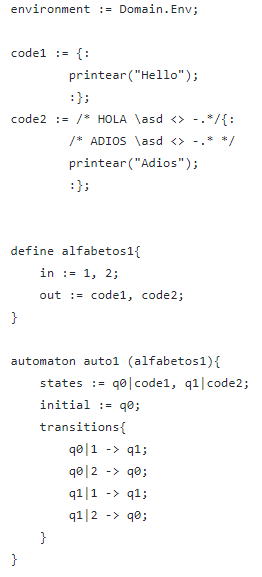
\includegraphics[width=7cm]{Mooma_Example.png}
	\caption{Ejemplo de Máquina de Moore usando Mooma.}
	\label{fig:MoomaExample1}
\end{figure}
\subsection{Compilando Mooma}
En nuestro caso, realizaremos el análisis de Mooma con dos herramientas completamente diferente:
\begin{itemize}
    \item En el caso de ANTLR4 nos encontramos ante una implementación en Python (lenguaje interpretado), por lo que su diagrama de T es de la forma [\ref{fig:pythonDiagrama}].
    \item En el caso de JFlex+Cup, nos encontramos con implementaciones en Java (lenguaje compilado e interpretado en máquina virtual), su diagrama de T es de la forma [\ref{fig:flexcupDiagrama}].
\end{itemize}
\begin{figure}[htb]
	\centering
	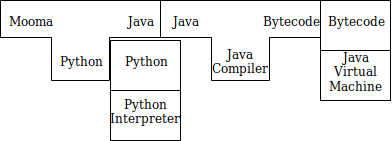
\includegraphics[width=8cm]{antlr.png}
	\caption{Diagrama de T para ANTLR4.}
	\label{fig:pythonDiagrama}
\end{figure}
\begin{figure}[htb]
	\centering
	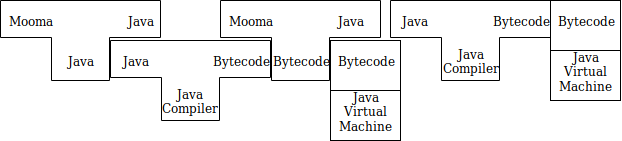
\includegraphics[width=12cm]{cup.png}
	\caption{Diagrama de T para jflex y cup.}
	\label{fig:flexcupDiagrama}
\end{figure}
Ambos analizadores tienen el mismo objetivo, generar código java con la Máquina de Moore implementada, por lo que podemos apreciar como la parte derecha de ambos diagramas [\ref{fig:pythonDiagrama}, \ref{fig:flexcupDiagrama}] son idénticas, ya que generarán el mismo código Java que debe ser compilado e interpretado por su máquina virtual finalmente.
\section{Analizador usando ANTLR}
ANTLR es un procesador de lenguaje que toma como entrada una gramática, escrita en un archivo en el lenguaje propio de ANTLR con extensión \textit{.g4}, y da como resultado un analizador léxico y un analizador sintáctico descendente implementado mediante funciones recursivas. Estos analizadores, para los cuales podemos escoger un lenguaje de programación de salida (En nuestro caso \textbf{Python3}), son fácilmente integrables en cualquier programa, y nos dejaría con la única responsabilidad de construir la parte de análisis semántico.

\subsection{Gramática ANTLR}
Para construir un procesador de lenguajes con ANTLR lo primero que tenemos que hacer es escribir nuestra gramática en formato \textit{.g4}. La gramática completa se puede ver en el archivo mooma.g4. A continuación vamos a discutir los aspectos más importantes:
\\

La gramática ANTLR se divide en 2 tipos de reglas: Las reglas léxicas y las reglas sintácticas. Las reglas léxicas, aquellas reglas que empiezan por mayúscula, sirven para definir los tokens que el \textit{lexer} va a analizar, y los que usaremos como terminales en la parte de las reglas sintácticas. Estas reglas sintácticas, escritas empezando por minúscula, son las que denotan la estructura del programa, y las que el \textit{parser} utilizará para realizar su análisis sintáctico.


\begin{figure}[htb]
	\centering
	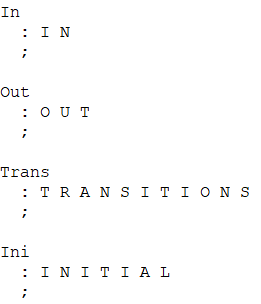
\includegraphics[width=5cm]{lexerRulesReserved.png}
	\caption{Reglas léxicas para tokens de palabras reservadas.}
	\label{fig:lexerRR}
\end{figure}

\begin{figure}[htb]
	\centering
	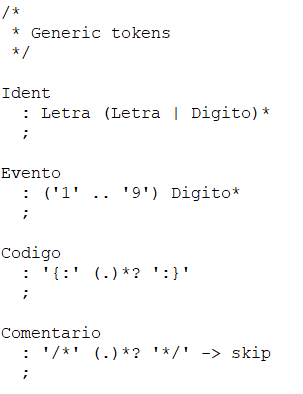
\includegraphics[width=6cm]{lexerRules.png}
	\caption{Reglas léxicas para algunos de los tokens utilizados.}
	\label{fig:lexerR}
\end{figure}

\begin{figure}[htb]
	\centering
	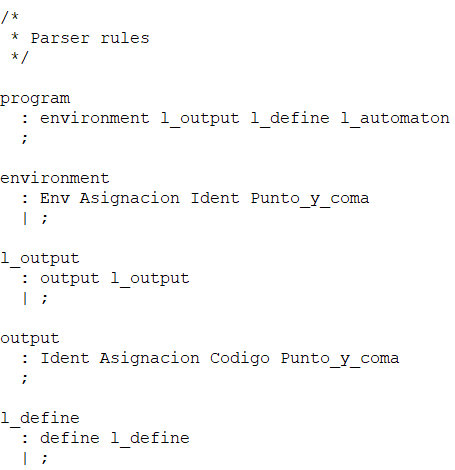
\includegraphics[width=8cm]{parserRules.png}
	\caption{Ejemplo de reglas sintácticas.}
	\label{fig:ParserR}
\end{figure}

Es importante notar que, debido a la gramática que hemos utilizado, podemos reconocer las palabras reservadas tanto en letra minúscula como en mayúscula, , incluso alternando estas (e.g. ``EnvIroNMent'' se reconocería correctamente como el token ``environment'') y no se puede definir el evento 0.

Aunque ANTLR es capaz de solucionar por sí solo las conflictos entre iniciales de la gramática, hemos decidido aplicar lo aprendido en clase y solucionarlo nosotros. Esto resulta en una gramática más compleja y difícil de manejar en la etapa semántica.
\\

Una vez hemos terminado de escribir nuestra gramática, ejecutamos la herramienta de ANTLR de la siguiente manera (Se usa la estructura de directorios de nuestro repositorio):
\begin{lstlisting}[caption=Ejecución de ANTLR.]
java -jar .\lib\antlr-4.7.1-complete.jar -Dlanguage=Python3 .\Lenguaje\mooma.g4
\end{lstlisting}

El argumento \textit{-DLanguage=Python3} se usa para elegir el lenguaje objeto de ANTLR, en nuestro caso Python3. La ejecución del anterior comando nos genera multitud de archivos, entre los que se encuentran el \textit{lexer} y el \textit{parser} que nos interesan. Ahora solo necesitamos escribir un pequeño programa que sirva para utilizarlos, como el siguiente:

\begin{lstlisting}[caption=Programa Main para la ejecución de los analizadores léxico y sintáctico., language=Python]
def main(args):
    file = FileStream(args.input_file)

    errorListener = moomaErrorListener()

    lexer = moomaLexer(file)
    stream = CommonTokenStream(lexer)
    parser = moomaParser(stream)
    parser.removeErrorListeners()
    parser.addErrorListener(errorListener)
    tree = parser.program()

    args.output = os.path.abspath(args.output)
    if not os.path.isdir(args.output):
        sys.stderr.write("Directory not found: {}\n".format(args.output))
        sys.exit(2)

    listener = MyMoomaListener(args.output)
    walker = ParseTreeWalker()
    walker.walk(listener, tree)

    write_parsed_to_file(listener, args.package)

    listener.file.close()
\end{lstlisting}

En este programa se pueden apreciar varias cosas: Es necesario crear un objeto \textit{lexer} y un objeto \textit{parser}. Esto hay que hacerlo en cualquier programa que utilice ANTLR. También se puede notar cómo usamos un listener de error personalizado, y un listener llamado \textbf{MyMoomaListener}, el cuál es el encargado de realizar el análisis semántico y del cuál hablaremos a continuación.

\subsection{Análisis semántico}
\subsubsection{Funcionamiento general con ANTLR}
ANTLR funciona realizando un análisis semántico con árbol de análisis sintáctico (Aunque también presenta la posibilidad de añadir acciones semánticas a la gramática descrita anteriormente, realizando el análisis semántico con un método sin recuerdo). El \textit{parser} da como resultado un objeto de tipo \textit{ParseTree}, el cuál recorremos con el mecanismo que ANTLR nos proporciona, llamado \textit{ParseTreeWalker} (líneas 19 y 20 del programa anterior). Este método realiza un recorrido en profundidad del árbol sintáctico, y utiliza un \textit{listener} para ejecutar la acción semántica que nosotros queramos en cada nodo del árbol. 

El modo que tiene ANTLR de funcionar semánticamente es el siguiente: Para cada regla sintáctica definida habrá dos funciones, una de entrada y una de salida. Estas funciones se ejecutarán al visitar un nodo de esa regla sintáctica. Por ejemplo: tenemos una regla sintáctica llamada automaton y que denota la estructura de una construcción \textit{Automaton}. 

\begin{lstlisting}[caption=Regla sintáctica automaton.]
automaton
  : Auto Ident Par_izquierdo Ident Par_derecho Llave_izquierda states initial transitions Llave_derecha
  ;
\end{lstlisting}

El \textit{listener} que nosotros entremos tendrá acceso a las siguientes 2 funciones:
\begin{itemize}
    \item enterAutomaton: se ejecuta cuando el recorrido del árbol llegue al nodo \textit{automaton}.
    \item exitAutomaton: se ejecuta cuando todos los nodos hijos de \textit{automaton} hayan sido evaluados.
\end{itemize}

Habrá tantas funciones de entrada y salida como reglas \textbf{sintácticas} tengamos. Las reglas léxicas no tienen acceso a estas funciones, siendo los tokens definidos \textbf{propiedades} de cada nodo. En nuestro ejemplo anterior, el nodo \textit{automaton} tendrá las propiedades Auto, Ident, Par\_izquierdo Par\_derecho Llave\_izquierda y Llave\_derecha, siendo el valor de cada una el lexema del token al que refieren. 

\subsubsection{Implementación del analizador semántico Mooma}

Para conseguir recoger toda la información necesaria para acabar escribiendo el archivo Java que queremos como resultado, hemos decidido realizar una aproximación orientada a objetos, teniendo las clases Lenguaje, Automata y Transición. Construiremos objetos cada vez que nos encontremos con una construcción en nuestro archivo de entrada, teniendo al final una lista de lenguajes y automatas, cada uno con la información que contienen en el archivo ''.moo''. 

A continuación un ejemplo de función, en la cual creamos un objeto de la clase Lenguaje:

\begin{lstlisting}[caption=Función enterDefine., language=Python]
def enterDefine(self, ctx:moomaParser.DefineContext):
        # Check if a language identifier has already been defined
        if str(ctx.Ident()) in self.languages:
            self.error = True
            self.errorLog.append("Identificador de lenguaje ya definido: {}".format(str(ctx.Ident())))

            # Create dummy language
            self.languages.append(Language("Dummy"))
            self.languageError = True
        else:
            self.languages.append(Language(str(ctx.Ident())))
\end{lstlisting}

Como se puede ver, la mayor parte del código está compuesta por la comprobación de posibles errores semánticos, de los cuales hablaremos más adelante.

El analizador acabará escribiendo en el archivo Machines.java los autómatas definidos en el archivo fuente, si no ha habido ningún error, junto con todos los archivos necesarios para la ejecución de los autómatas, dejando al usuario la responsabilidad de crear un programa que utilice los autómatas. En caso de error o errores, se escribirá por pantalla la lista de errores encontrados.

\subsection{Detección de errores}
\subsubsection{Errores en el análisis léxico y sintáctico}
El análisis léxico y semántico se realiza mediante los analizadores generados automáticamente por ANTLR, pero aún así podemos modificar cómo se trata el error. 

Por defecto, ANTLR comprueba los errores del \textit{lexer} y del \textit{parser} mediante lo que llama como \textit{ErrorListener}. Este listener tiene funciones que se llaman cuando ese error ocurre. La que más nos interesa es \textit{SyntaxError}. Aunque su nombre indique que se llama cuando el \textit{parser} encuentra un error, esta funcion también se llama en la fase del análisis léxico cuando se encuentra un token mal formado. La información que nos proporciona consiste en la línea y columna en la que el error se ha encontrado, así como un mensaje de error bastante descriptivo del error. El siguiente mensaje se puede replicar si se intenta procesar el archivo "test2.moo" de nuestro repositorio.

\begin{lstlisting}[caption=Mensaje de error para test2.moo.]
line 19:0 no viable alternative at input '}'
}
^
\end{lstlisting}

Se ha optado por personalizar un poco el mensaje de error que da el \textit{ErrorListener} por defecto, añadiendo la línea de error con la parte conflictiva, como se puede ver en el siguiente ejemplo (Sta es el nombre del token \textit{states)}:

\begin{lstlisting}[caption=Mesaje de error para un token mal formado.]
line 43:4 mismatched input 'stes' expecting Sta
    stes := estate1|code1, estate2|code2, estate3|code2;
    ^^^^
\end{lstlisting}

\subsubsection{Errores en el análisis semántico}
Además de recuperar toda la información semántica para generar los archivos Java necesarios, el analizador semántico también necesita comprobar que ciertos errores no han sido cometidos que son imposibles de encontrar en el análisis léxico y sintáctico. Los errores que se comprueban en nuestro analizador semántico son:
\begin{itemize}
    \item Identificadores de código de salida repetidos.
    \item Identificadores de lenguaje repetidos.
    \item Evento repetido en un lenguaje.
    \item Identificador de salida repetido en un lenguaje.
    \item Identificador de autómata repetido.
    \item El identificador de lenguaje asociado a un autómata no ha sido definido.
    \item Identificador de estado repetido en un mismo autómata.
    \item El identificador de salida asociado a un estado no existe en el lenguaje de salida del autómata.
    \item El estado inicial no es un estado del autómata.
    \item El estado de origen o de destino de una transición no es un estado del autómata.
    \item El evento de una transición no forma parte del lenguaje de entrada.
\end{itemize}

\vspace{10mm}
Si cualquiera de estos errores ocurre, el análisis no para. Al final del análisis se mostrarán por pantalla todos los errores semánticos que han ocurrido, y no se generará ningún archivo Java.

\section{Analizador usando Flex+Cup}
\subsection{Análisis Léxico}
Hemos realizado el análisis léxico usando JFlex, esta parte solo se encarga de reconocer cada uno de los tokens de [\ref{tab:Tokens}] de forma que serán la entrada del análisis sintáctico que hemos realizado en Cup. El reconocimiento de estos tokens se ha realizado mediante expresiones regulares, de forma análoga a como se ha visto en clase.

De esta parte cabe destacar que las palabras reservadas son reconocidas tanto en letra minúscula como mayúscula (Igual que en el analizador construido con ANTLR). Además, en esta parte, al reconocer cada uno de los tokens ya se indica su tipo de dato (en Java), en nuestro caso todos los tokens se pasan al analizador sintáctico como tipo String.

\subsection{Analizador Sintáctico+Semántico}
En este caso, con cup realizamos un análisis sintáctico ascendente, la gramática usada es exactamente la misma que usamos en el analizador descendente de ANTLR4. Podríamos haber creado una gramática distinta ya que en este caso la recursividad a izquierda no es un problema, pero por simplicidad hemos decidido mantenerla.

Cup realiza el análisis semántico al mismo tiempo que el sintáctico, de forma que a las producciones de la gramática hay que añadirles unas reglas semánticas para dar significado a dichas producciones. En nuestro caso (en el archivo moomaParser.cup) el funcionamiento es sencillo, tenemos unas estructuras globales (a nivel de clase) en las que las producciones irán almacenando información de la máquina, para, al reducir por la producción ``program'', esta información sea escrita en su respectivo archivo ``Machines.java'' con la sintaxis de java correcta. Además, al reducir la producción inicial también se escriben los archivos auxiliares de los que depende el correcto funcionamiento de la Máquina de Moore.

Algunas de las producciones que almacenan la información en dichas estructuras globales son las siguientes:
\begin{lstlisting}[caption=Producción transition.]
l_transitions
  ::= IDENT:i SEPARATOR l_evento:e FLECHA IDENT:c PUNTO_Y_COMA l_transitions {:
    String [] s = new String [3];
    s[0]=i;
    s[1]=c;
    s[2]=e;
    transitions.add(s);:}
  | ;
\end{lstlisting}
Se puede apreciar como se crea un Array de String, donde se guardan los identificadores (estado origen y estado destino) y el evento que debe ocurrir para realizar dicha transición, posteriormente este array se almacena en la lista global.
\begin{lstlisting}[caption=Producción states.]
l_states
  ::= IDENT:i SEPARATOR IDENT:c l_states_fact {:  String [] s = new String [2];
    s[0]=i;
    s[1]=c;
    states.add(s);:}
  ;
 \end{lstlisting}
 De forma análoga ocurre en esta producción, el identificador del estado y su salida se almacenan en un array, que a su vez se almacena en la lista global.
 \begin{lstlisting}[caption=Producción program.]
program
  ::= environment:env l_output l_define l_automaton {:
  writeAuxiliar(env);
  try {
    writer = new PrintWriter("Machines.java", "UTF-8");
  }catch( Exception e){
    e.printStackTrace();
  }
  writer.println(String.format("package %s;\n\n",env));
  writer.println("public class Machines {\n");
  for(int i=0;i<automatons.size();i++){
    writer.println(String.format("\tpublic static IMooreMachine %s(){\n\t\tMooreMachine machine = new MooreMachine();\n\t\tmachine.setMachineName(\"%s\");",automatons.get(i),automatons.get(i)));
    for(int j=0;j<states.size();j++){
      String out = "";
      for(int k=0;k<outputs.size();k++){
        if(outputs.get(k)[0].equals(states.get(j)[1])){
          out=outputs.get(k)[1];
          out=out.replace("\n","\n\t\t");
          break;
        }
      }
      writer.println(String.format("\n\t\tState %s = new State(\"%s\");\n\t\t%s.setOutput(() -> {%s});\n\t\tmachine.addState(%s);",states.get(j)[0],states.get(j)[0],states.get(j)[0],out.substring(2,out.length()-2),states.get(j)[0]));
    }
    int tranCount = 0;
    for(int j=0;j<transitions.size();j++){
      tranCount+=1;
      writer.println(String.format("\n\t\tTransition t%d = new Transition (%s,%s,\"%s\");\n\t\tmachine.addTransition(t%d);",tranCount,transitions.get(j)[0],transitions.get(j)[1],transitions.get(j)[2],tranCount));
    }
    writer.println(String.format("\n\t\tmachine.setInitialState(%s);",initial));
    writer.println("\n\t\treturn machine;\n\t}");
  }
  writer.println("\n}");
  writer.close();
  :}
  ;
\end{lstlisting}
La producción ``program'' es la más importante, ya que se puede observar como al reducir crea el archivo ``Machines.java'' que es el \emph{core} de la Máquina de Moore, se puede apreciar como en cada String que escribimos en el fichero se formatea la información almacenada en las estructuras globales para que se cree el archivo correctamente.

\subsection{Uso de las herramientas flex y cup}
El uso de estas herramientas es muy sencillo, una vez escrito nuestro archivo .mooma para la creación de la Máquina de Moore deseada seguimos los siguientes pasos:
\begin{itemize}
    \item Metemos el archivo mooma en el mismo directorio que los programas flex y cup.
    \item También es necesario introducir en el directorio el environment (el archivo .java que hereda de la interfaz que proporcionamos) que hayamos creado, y el directorio en cuestión debe tener el mismo nombre que el susodicho environment.
    \item Ejecutamos el comando para crear el analizador léxico: \begin{lstlisting}
jflex moomaLexer.flex
\end{lstlisting}
    \item Ejecutamos el comando para crear el analizador sintáctico y semántico:
    \begin{lstlisting}
java java_cup/Main moomaParser.cup
\end{lstlisting}
    \item Compilamos los analizadores:
    \begin{lstlisting}
javac analex.java parser.java Main.java sym.java
\end{lstlisting}
    \item Analizamos el archivo mooma:
        \begin{lstlisting}
java Main [Nombre].moo
\end{lstlisting}
    \item Compilamos todos los nuevos archivos generados:
    \begin{lstlisting}
javac *.java
\end{lstlisting}
    \item Ejecutamos nuestro programa principal para que empiece a funcionar nuestra Máquina de Moore.

\end{itemize}

\section{Ejemplos de uso}
El procesador de lenguaje que hemos construido genera una multitud de archivos Java para el modelado y simulación de máquinas genéricas de Moore, pero es necesario integrarlas en un programa que el usuario debe escribir. Además es necesario que implemente la interfaz \textit{Environment} para que la simulación pueda ocurrir. Por eso, vamos a enseñar varios ejemplos de uso.

\subsection{PredictionBuffer} \label{sec:predbuff}
En el dominio de los procesadores y el lenguaje máquina, muchas veces el procesador se va a encontrar con una instrucción condicional de salto. En estos casos, el procesador debe tomar el riesgo e intentar predecir si el salto se va a realizar o no. Esto es mejor que esperar a que la condición se resuelva, porque en caso de acertar, nos hemos ahorrado numerosos ciclos de reloj, aunque si se falla la predicción hemos perdido ciclos.

Una de las técnicas más báscias de predcción dinámica de salto es el uso del \textbf{buffer de predicción}. Se mantienen 2 bits con los resultados de los dos últimos saltos y su resultado. Esto se puede modelar mediante una máquina de Moore como se puede ver en la Figura \ref{fig:PB}.

\begin{figure}[htb]
	\centering
	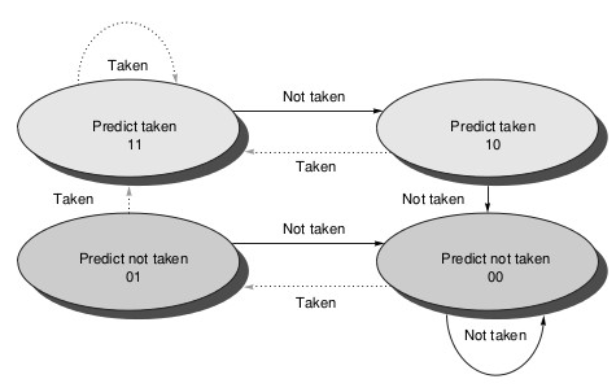
\includegraphics[width=12cm]{figures/PredictionBuffer.png}
	\caption{Autómata de Buffer de predicción.}
	\label{fig:PB}
\end{figure}

En esta máquina tendríamos 4 estados, 2 posibles entradas (''Taken'' y ''Not Taken'') y dos posibles salidas (''Predicción de salto'' y ''Predicción de no salto''). Para generar la máquina de Moore con nuestro procesador de lenguaje, el archivo ''.moo'' quedaría de la siguiente manera:

\begin{lstlisting}[caption=PredictionBuffer.moo.]
/* 
Prediction Buffer para 2 bits
*/

environment := Env ;

code1 := {: 
        Env.predictTaken()
        :};
code2 := {:
        Env.predictNotTaken()
        :};


define alfabeto1{
    in := 1, 2;
    out := code1, code2;
}

automaton automata1 (alfabeto1){
    states := q0|code2, q1|code2, q2|code1, q3|code1;
    initial := q2;
    transitions{
        q0|1 -> q0;
        q0|2 -> q1;
        q1|1 -> q0;
        q1|2 -> q2;
        q2|1 -> q3;
        q2|2 -> q2;
        q3|1 -> q0;
        q3|2 -> q2;
    }
}
\end{lstlisting}

El \textit{Environment} para el ejemplo es el siguiente:

\begin{lstlisting}[caption= Environment para el autómata anterior., language=Java]
public class Env implements IEnvironment {

	@Override
	public String translate(Object input) {
        if (input.toString().equals("Taken")){
            return "2";
        }
        else if (input.toString().equals("Not Taken")){
            return "1";
        }
        else{
            return "0";
        }
	}
    
    public static void predictTaken(){
        System.out.println("Predecimos salto");
    }
    
    public static void predictNotTaken(){
        System.out.println("Predecimos no salto");
    }

}
\end{lstlisting}

Aquí se puede ver el uso de la clase \textit{Environment}. Mediante el método \textit{translate} convertimos las entradas ''Taken'' y ''Not Taken'' en eventos. Además podemos implementar funciones que luego serán referenciadas en los códigos de salida del archivo ''PredictionBuffer.moo''. En este ejemplo solo muestran un mensaje por pantalla, pero el usuario puede hacer tantas funciones como quiera, y puede hacerlas tan complejas como quiera.


Una vez tenemos el \textit{Environment} y el ''PredictionBuffer.moo'', solo tenemos que ejecutar el procesador de lenguaje, que nos generará varios archivos Java. Para que todo funcione, tenemos que escribir un programa que integre la máquina de Moore. Un programa básico que hemos escrito para este ejemplo es el siguiente:
\begin{lstlisting}[caption= Main para el autómata anterior.]
import java.util.Scanner;
public class Main {
    public static void main(String[] args){
        Scanner sc = new Scanner(System.in);
        MachineController mc = new MachineController(Machines.automata1());


        System.out.print("Input: ");
        String input = sc.nextLine();

        while(!input.equals("")){
            if (mc.addNewInput(input) != null){
                mc.getCurrentState().getOutput().accept(mc.getEnvironment());
            }
            else{
                System.out.println("Entrada no reconocida por el automata");
            }
            System.out.print("Input: ");
            input = sc.nextLine();
        }

        sc.close();
    }
}
\end{lstlisting}
Como se puede comprobar, solo es necesario crear un \textit{MachineController}, pasándole como argumento la máquina de Moore que va a usar. El programa entra en un bucle para seguir tomando entradas para la máquina por la entrada estándar, y ejecuta el código de salida llamando al método \textit{accept}, el cual necesita como argumento el entorno.

\subsection{IA de enemigos en un videojuego}
Los motores de juegos más populares, \emph{Unity} y \emph{Unreal Engine 4}, traen incorporado un módulo de IA que permite dotar a los enemigos del jugador de un comportamiento autónomo. Este comportamiento se modela a través de árboles de comportamiento. Un ejemplo de árbol de comportamiento se puede ver en la figura \ref{fig:UE4BT}

\begin{figure}[h]
    \centering
    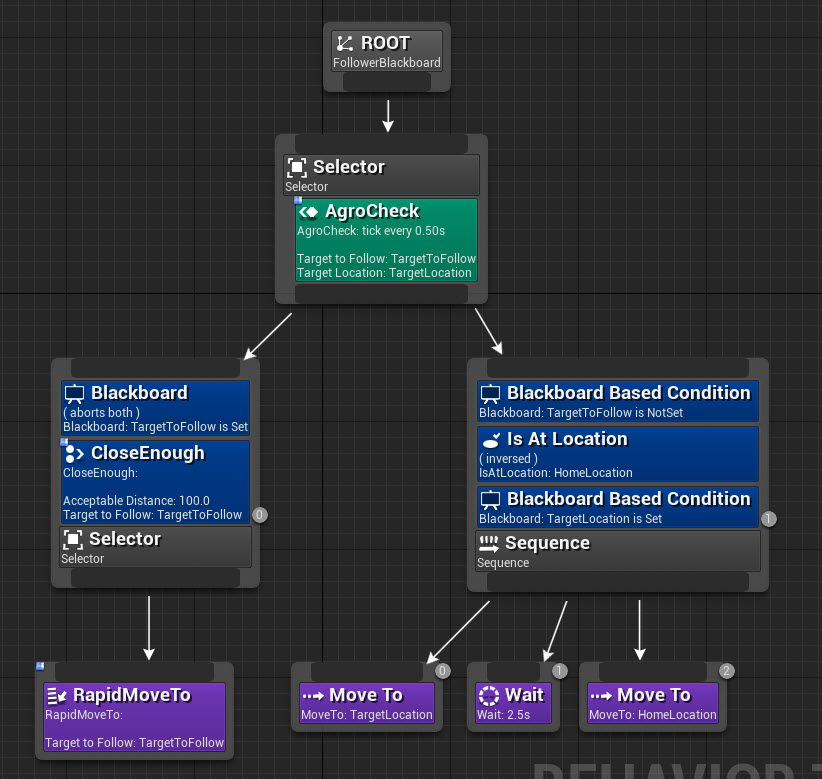
\includegraphics[width=10cm]{figures/UnrealBehaviourTree.jpg}
    \caption{Ejemplo de Árbol de Comportamiento en \emph{Unreal Engine 4}}
    \label{fig:UE4BT}
\end{figure}

Sin embargo, esta no es la única forma de modelar un comportamiento autónomo, estos comportamientos también se pueden modelar mediante una máquina de Moore.

En este ejemplo se ha modelado el comportamiento de un enemigo que ataca cuerpo a cuerpo y que prioriza el no ser atacado sobre el dañar a su enemigo (el jugador) \ref{fig:state_machine_ia}.

\begin{figure}[b]
    \centering
    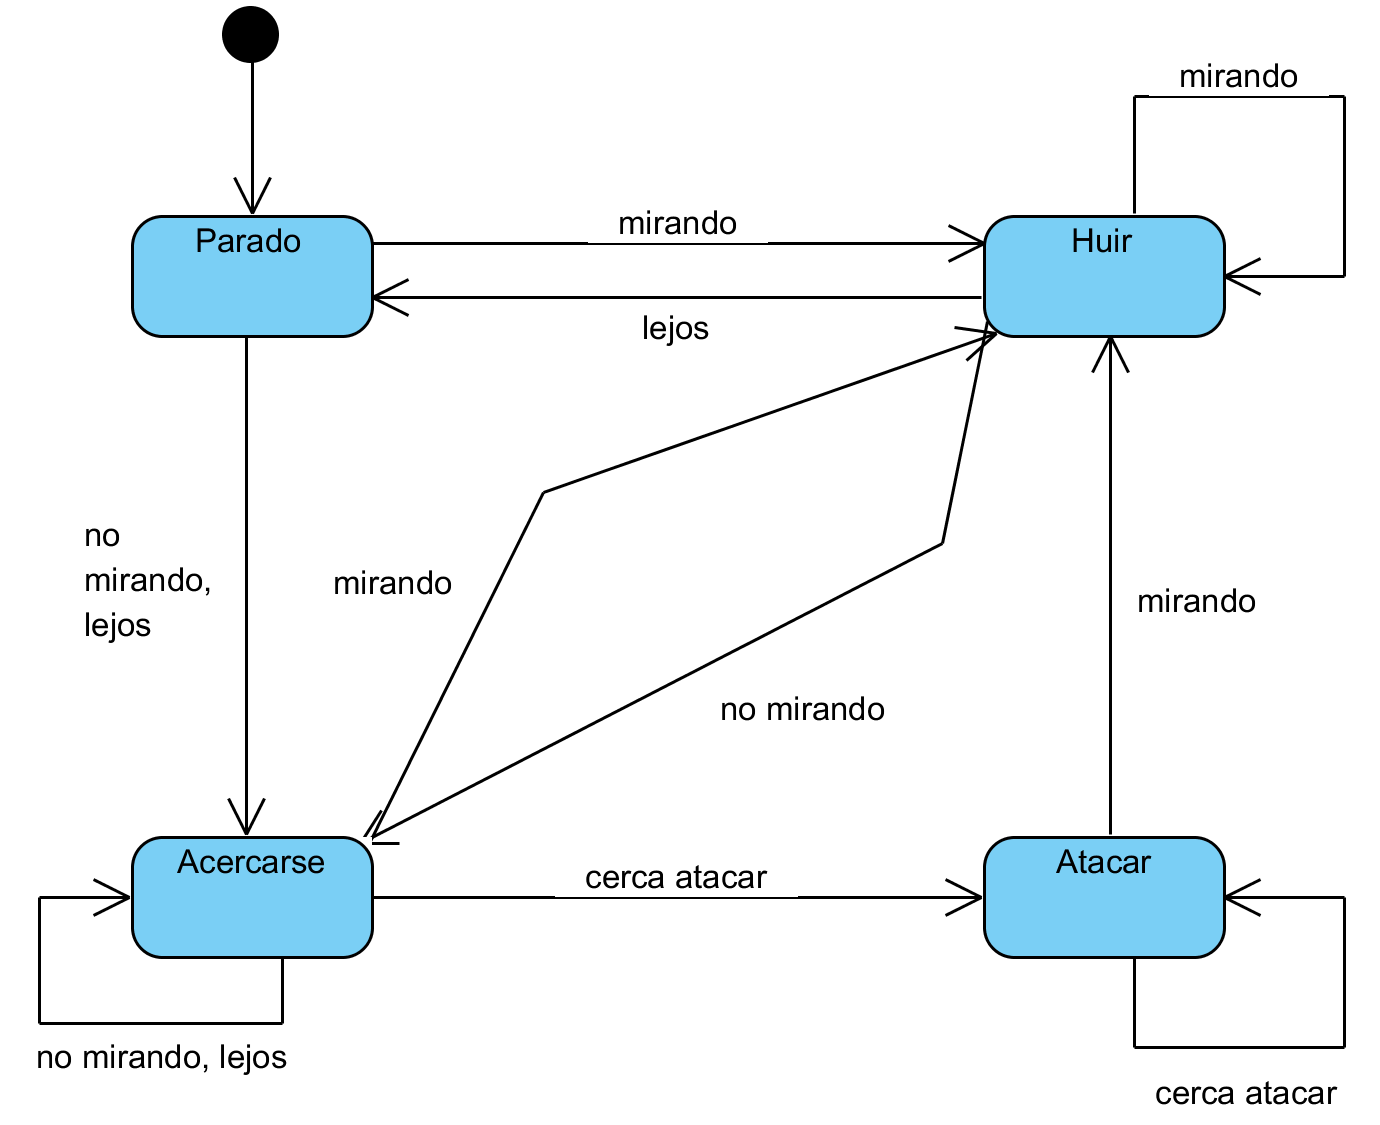
\includegraphics[width=10cm]{figures/statemachineia.png}
    \caption{Máquina de estado del ejemplo GameIA}
    \label{fig:state_machine_ia}
\end{figure}

La máquina, traducida al lenguaje \emph{Mooma} está representada en el listado \ref{lst:gameiamooma}

\begin{lstlisting}[caption=GameIA.moo, label=lst:gameiamooma]
/* IA de un enemigo en un videojuego */

environment := GameAIEnvironment;

code1 := {: env.notify("Huir") :};
code2 := {: env.notify("Parado") :};
code3 := {: env.notify("Andar") :};
code4 := {: env.notify("Atacar") :};


define EnemyAlphabet {
    in := 1, 2, 5, 10; /* Mirando, No Mirando, Lejos, Cerca Atacar */
    out := code1, code2, code3, code4;
}

automaton MeleeEnemy (EnemyAlphabet){
    states := Huir|code1, Parado|code2, Andar|code3, Atacar|code4;
    initial := Parado;
    transitions{
        Parado|1 -> Huir;
        Parado|2 -> Andar; Parado|5 -> Andar;
        Huir|5 -> Parado;
        Huir|1 -> Huir;
        Huir|2 -> Andar;
        Andar|2 -> Andar; Andar|5 -> Andar;
        Andar|1 -> Huir;
        Andar|10 -> Atacar;
        Atacar|1 -> Huir;
        Atacar|10 -> Atacar;
    }
}
\end{lstlisting}

Como podemos ver en la línea 12 del listado \ref{lst:gameiamooma} se ha tenido que traducir las entradas del autómata por eventos numéricos.

En el archivo se menciona la clase \emph{GameAIEnvironment}, el entorno de la máquina de Moore, representada en el listado \ref{lst:gameaienv}

\begin{lstlisting}[caption=GameIA.moo, label=lst:gameiamooma, language=Java]
public class GameAIEnvironment implements IEnvironment {
    private HashMap<String, List<Runnable>> listeners;
    
    public GameAIEnvironment() {
        listeners = new HashMap<>();
    }
    
    public void notify(String state) {
        if (listeners.containsKey(state)) {
            listeners.get(state).forEach((Runnable action) -> action.run());
        }
    }
    
    public void addListener(String state, Runnable action) {
        if (!listeners.containsKey(state))
            listeners.put(state, new LinkedList<>());
        
        listeners.get(state).add(action);
    }
    
    public String translate(Object input) {
        return input.toString();
    }
    
    public String translate(Enemy me, Character ch) {
        double angle = WorldCanvas.angleBetweenPoints(ch.getX(), me.getX(), ch.getY(), me.getY()) * -1;
        double distance = WorldCanvas.euclideanDistance(ch.getX(), me.getX(), ch.getY(), me.getY());
        
        if (distance >= Character.VISION_LENGTH)
            return "5";
        else if ((ch.getAngle() - Character.VISION_CONE / 2) <= angle && (ch.getAngle() + Character.VISION_CONE / 2) >= angle)
            return "1";
        else if (distance <= Enemy.ATTACK_RANGE)
            return "10";
        else
            return "2";
    }
}
\end{lstlisting}

Como se puede ver, este entorno es mucho más complejo que el del búfer de prediccion (sección  \ref{sec:predbuff}) ya que es necesario que el entorno interactúe con la interfaz. Para realizar esta interacción se ha optado por un diseño basado en el patrón \emph{Observer} aprovechando las características funcionales añadidas en \emph{Java 8}.

También es necesario que el entorno calcule distancias y ángulos para comprobar la condicion de \emph{mirando}, estas operaciones se delegan a la clase \emph{WorldCanvas} que es la encargada de la interfaz.

El código que ejecuta cada estado recibe una instancia de la clase \emph{IEnvironment}, gracias a esto es posible tener varias máquinas de Moore funcionando a la vez, ya que no se usan variables ni métodos estáticos.

Cada máquina de Moore tiene asociada una clase \emph{Pawn} que es la que se encarga de manejar el personaje dentro del mundo y interactuar con la máquina.

El diagrama de clases del ejemplo se puede ver en la figura \ref{fig:classdiagram} y el ejemplo de ejecución del ejemplo se puede ver en la figura \ref{fig:moomauiexample}.

\begin{figure}[]
    \centering
    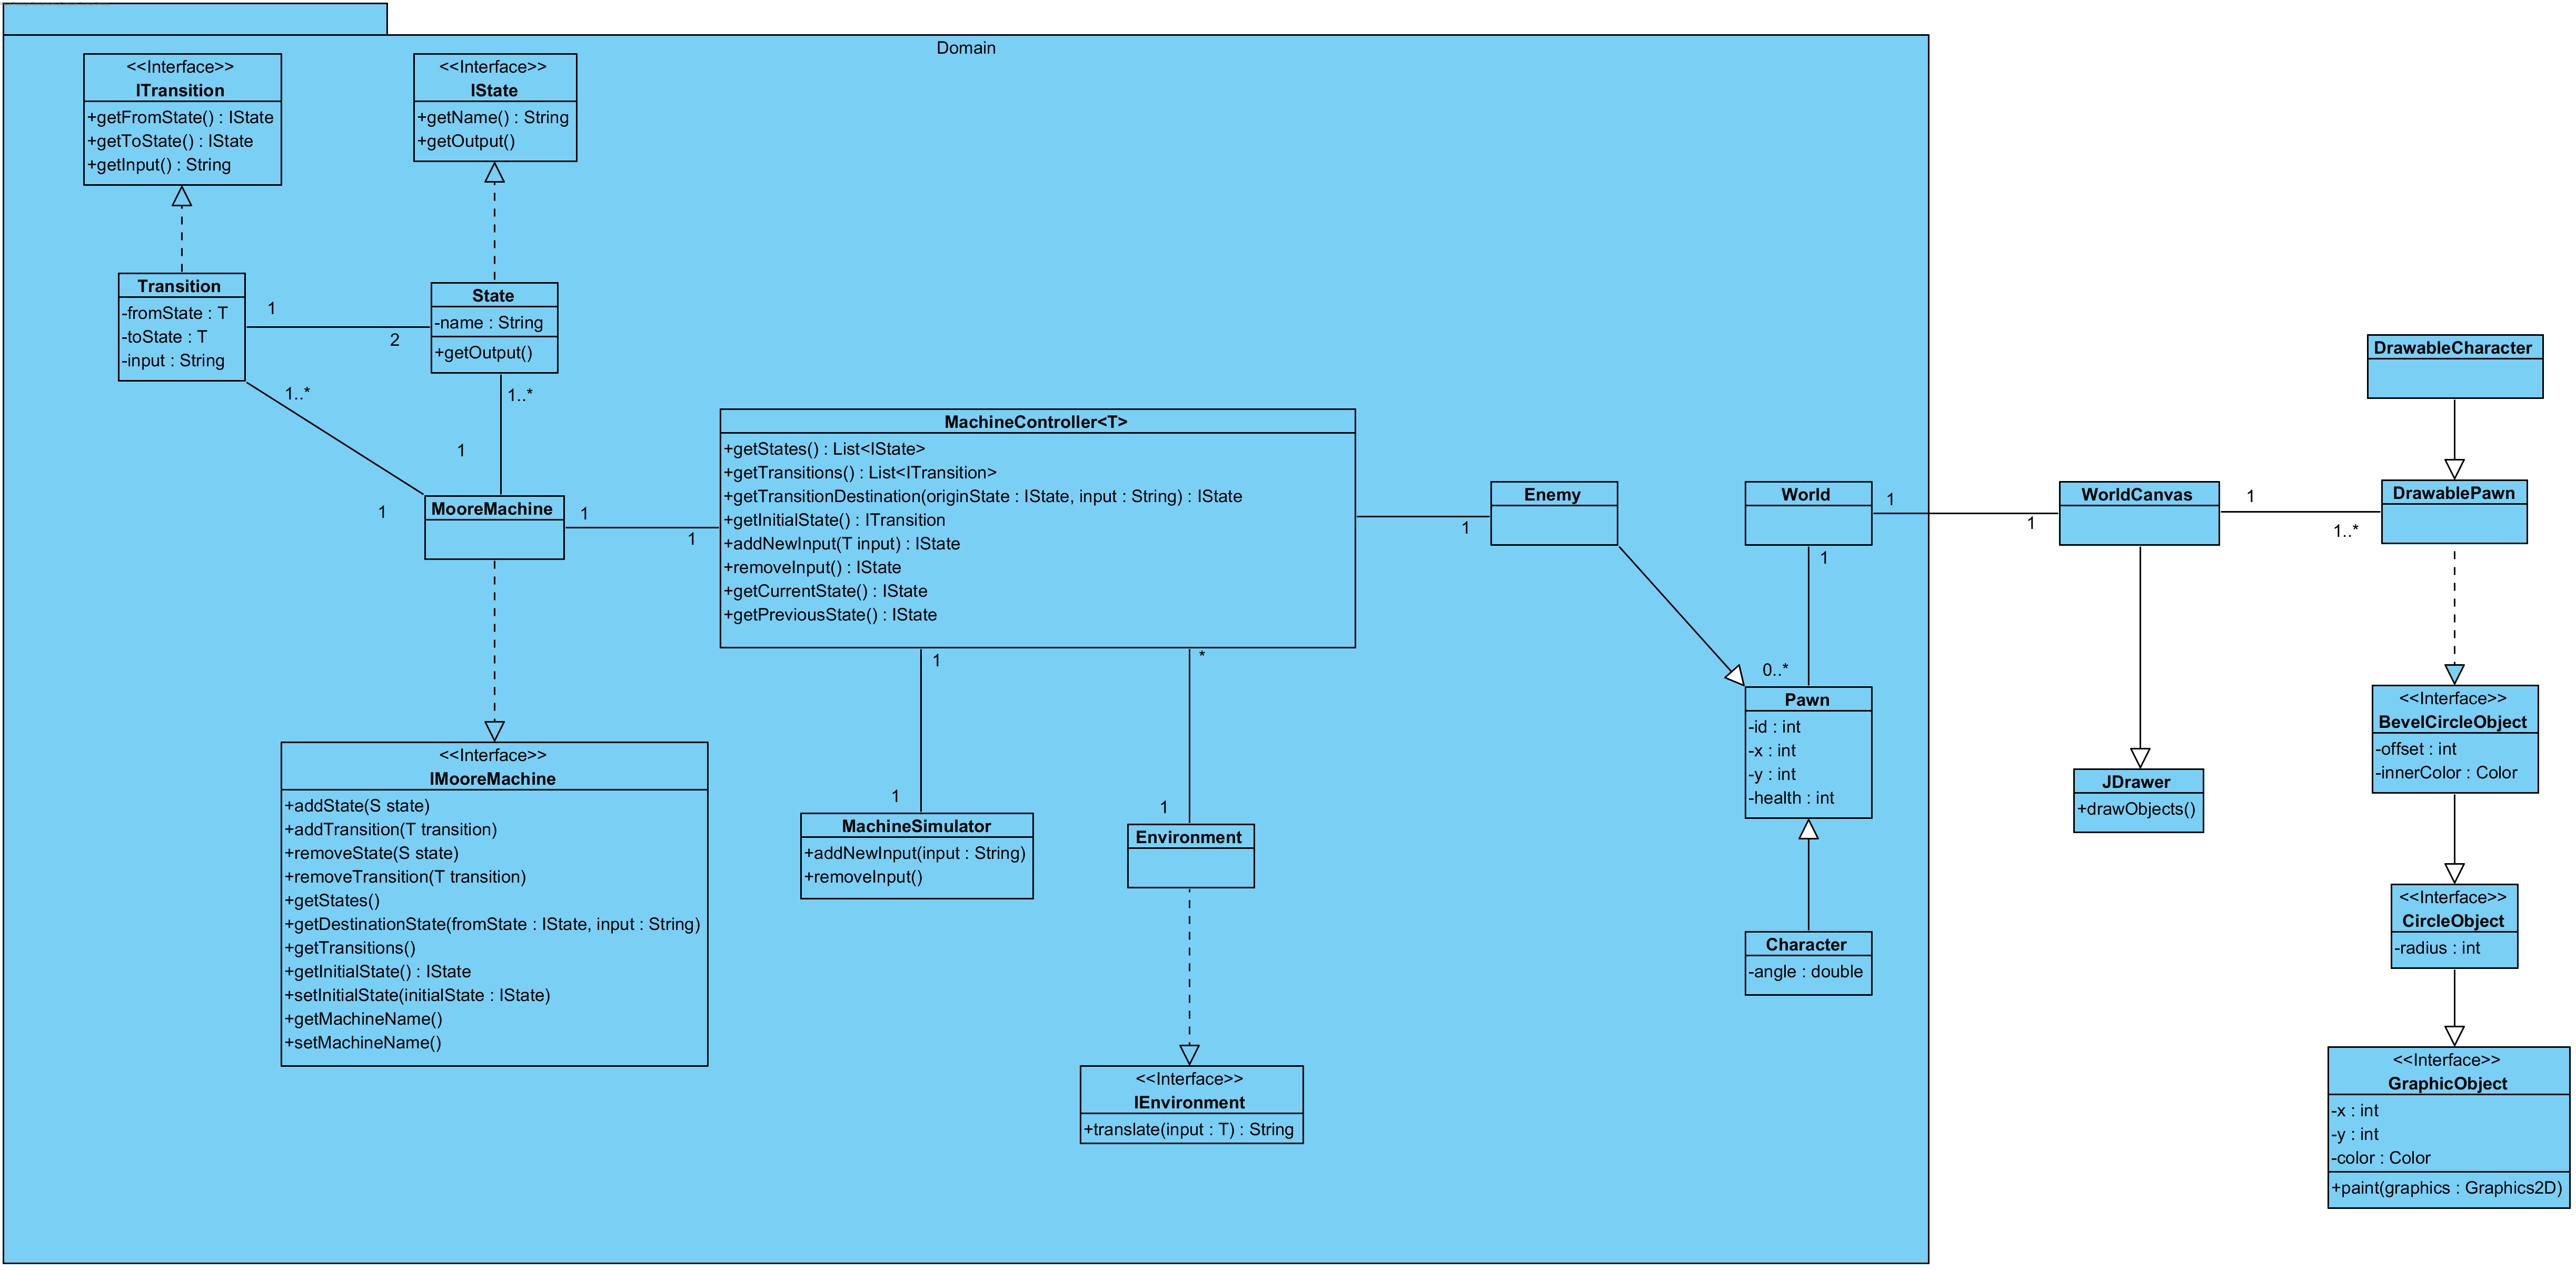
\includegraphics[width=\linewidth]{figures/classdiagram.png}
    \caption{Diagrama de clases del ejemplo GameIA}
    \label{fig:classdiagram}
\end{figure}

\begin{figure}[b]
    \centering
    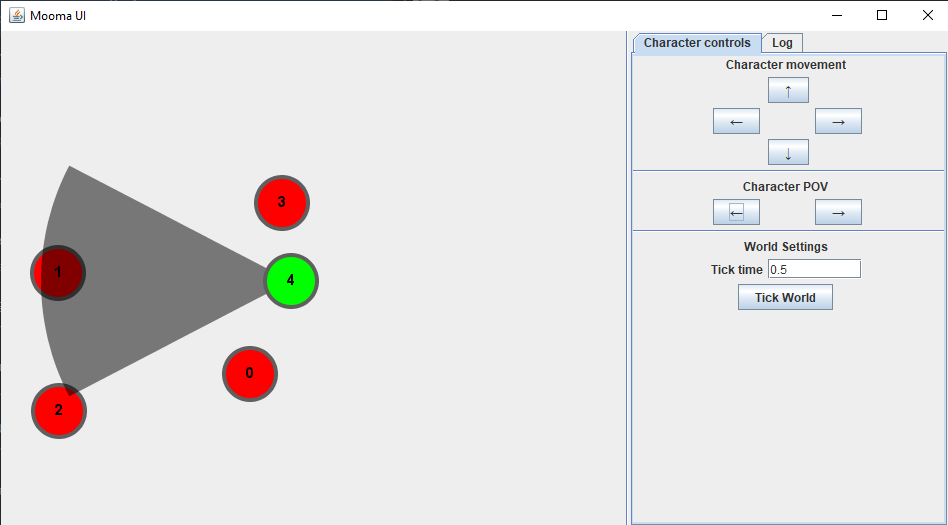
\includegraphics[width=\linewidth]{figures/moomauiexample.png}
    \caption{Ejemplo de ejecución del ejemplo GameIA}
    \label{fig:moomauiexample}
\end{figure}


\end{document}

% Local Variables:
% coding: utf-8
% mode: flyspell
% ispell-local-dictionary: "castellano8"
% mode: latex
% End:
